\section{Treinamento de modelo}

Treinamento de modelo para sugestão de posts para determinados conteúdos.

\subsection{LDA}

LDA é um algoritmo de aprendizagem não supervisionado que associa tópicos a documentos. Documentos são como textos e cada um pode conter mais de um tópico.
Tópicos são formados por palavras e uma mesma palavra pode fazer parte de mais de um tópico, ou seja, uma mesma palavra contribui para a formação de vários 
tópicos. Os tópicos são descobertos durante o treinamento do modelo mas a quantidade de tópicos deve ser especificada a priori.

Após o treinamento do modelo um documento tem uma distribuição discrete de tópicos e um tópico tem uma distribuição discreta de palavras. 

Como exemplo temos... COLOCAR AQUI EXEMPLO DE UM DOCUMENTO, SEUS TÓPICOS E AS PALAVRAS QUE COMPOEM O TÓPICO.

\begin{itemize}
    \item DÚVIDA: DEVO EXPLICAR COM MAIS DETALHES A IMPLEMENTAÇÃO DO LDA? ACREDITO QUE NÃO...
\end{itemize}

Há vários tipos de uso para o algoritmo LDA, como entender melhor o tipo de documento um determinado conjunto de palavras (notícias, artigo na wikipedia, 
negócios), quantificar as palavras mais usadas e mais importantes em um texto ou mesmo encontrar semelhanças e recomendações de documentos. 

Neste trabalho eu usei LDA para encontrar semalhança entre textos de acordo com os tópicos do modelo treinado e fazer recomendações com base em textos novos.

LDA não tem boa performance com documentos curtos, como tweets, por exemplo, pois ele infere parâmetros a partir da observação de palavras e se não há palavras
suficientes não há as condições necessárias para um bom aproveitamento.

LDA é um algoritmo que trabalha com modelos do tipo bag of words, ou seja, não há importância na ordem das palavras. Outros algoritmos funcionam bem com sentençãs
estruturadas.

\subsubsection{Hiperparâmetros}

\begin{itemize}
    \item $\alpha$: Um valor baixo indica que documentos contém poucos tópicos contribuindo para os mesmos
    \item $\eta$: Um valor baixo indica que tópicos contém poucas palavras contribuindo para os mesmos, enquanto em um valor alto pode haver maior sobreposição 
    de palavras entre tópicos diferentes
\end{itemize}

\subsection{Cálculo de coerência}

Um dos parâmetros mais importantes para o algoritmo LDA é o número de tópicos escondidos que devem ser extraídos do corpus de treinamento.

Sendo o LDA um algoritmo não supervisionado é muito difícil validar se o conjunto de tópicos selecionados para um determinado conjunto de documentos
é útil e faz sentido. Não há uma lista de tópicos corretos previamente selecionados para comparar com os resultados obtidos. Uma forma de medir a 
eficiência do número de tópicos escolhidos é a **coerência**, que é uma avaliação quantitativa da qualidade dos tópicos aprendidos para um determinado 
conjunto de documentos.

Um conjunto de afirmações ou fatos é considerado coerente, se apoiarem um ao outro. Assim, um conjunto de fatos coerente pode ser interpretado 
em um contexto que cobre todos ou a maioria dos fatos. Um exemplo de conjunto de fatos coerentes é “o jogo é um esporte de equipe”, 
“o jogo é jogado com uma bola”, “o jogo exige grandes esforços físicos”.

A coerência de um tópico mede o grau de semelhança semântica entre as palavras que mais contribuem para a definição daquele tópico.
Esta medida ajuda a distinguir entre os tópicos que são \textbf{semanticamente interpretáveis} e os tópicos que são 
\textbf{artefatos de inferência estatística}.

Há várias medidas de coerência e a que escolhi foi a \textbf{c\_v}. Na lista de referências há artigos que explicam esta e outras 
medidas de coerência. O que importa é que um maior valor indica maior coerência.

\subsubsection{Análise de coerências}

Conforme podemos ver código fonte na seção seguinte, há alguns parâmetros importantes para o cálculo da coerência:

\begin{itemize}
    \item \textbf{documents}: lista de documentos que compôem nosso corpus
    \item \textbf{num\_topics}: número de tópicos para os quais queremos calcular a coerência
\end{itemize}

Apesar de não ser explicitamente utilizados no código, os parâmetros \textbf{alpha} e \textbf{eta} mencionados anteriormente são também importantes mas neste cálculo inicial
optei por mantê-los em seu valor padrão, que é 1/número de tópicos. 

A lista de documentos contempla o conjunto completo de textos de nossa fonte de dados de origem. O número de tópicos eu variei entre 5 e 120, de um 
a um. O resultado gerado foi um arquivo csv contendo os seguintes campos:

\begin{itemize}
    \item num\_topics: número de tópicos no Treinamento
    \item coherence: coerência para aquele número de tópicos
    \item tempo\_gasto: tempo total gasto no cálculo de coerência para o número de tópicos
\end{itemize}

Com base no resultado dos cálculos das coerências para o número de tópicos foi gerado o gráfico a seguir, onde já podemos ver que a coerência para 
de crescer e de certa forma e começa a oscilar para cima e para baixo sem grandes variações a partir de um determinado número de tópicos.

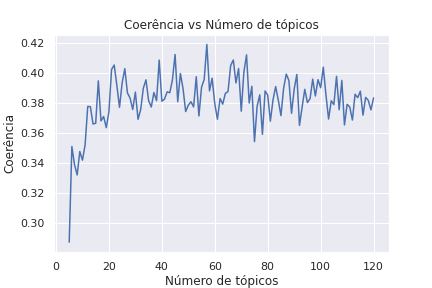
\includegraphics{coerencia_vs_topicos.png}

Ordenando os valores das coerências nós obtemos as dez maiores e seus respectivos tópicos, conforme vemos abaixo ordenando começando pela maior.

\begin{center}
\begin{tabular}{ |c|c| }
 \hline
 Número de tópicos & Coerência \\ [0.5ex]
 \hline\hline
 57 & 0.4187279439804192 \\
 45 & 0.4120513470103957 \\
 72 & 0.4118140382511174 \\
 67 & 0.4084148429857527 \\
 39 & 0.4083294457749056 \\
 22 & 0.4050952035903351 \\
 66 & 0.4047401968259075 \\
 101 & 0.4036451569534363 \\
 69 & 0.4027847252786048 \\
 26 & 0.4026587678111619 \\
 \hline
\end{tabular}
\end{center}

Abaixo segue uma listagem com o código fonte usado para o cálculo das coerências para um conjunto de documentos e intervalo de números de tópicos.

\subsubsection{Código fonte}

\lstinputlisting[language=Python, style=mystyle, frame=lines, caption=Código fonte: Cálculo de coerência de tópicos]{sourcecode/coerencia.py}

\subsection{Testes de análise de tópicos}

Após a definição de modelo com base nos documentos de origem foram feitos testes para avaliação de quais tópicos determinavam melhor os documentos e quais 
palavras definiam os tópicos com maior probabilidade. Como a execução deste algoritmo é não determinística as palavras (e seus id's) que definem 
um tópico pode ser alteradas de uma execução para outra. O resultado exibido aqui pode não ser o mesmo de execuções seguintes com os mesmos parâmetros mas 
o objetivo deste teste inicial é identificar palavras que estão contribuindo muito para definição dos tópicos mas que podem não ser interessantes 
para o objetivo de encontrar documentos semelhantes, então isto não é um problema.

A sequência de testes abaixo ilustra cenários de execução e está documentado o que foi feito até aquela cenário. A execução foi incremental, sendo que 
qualquer limpeza ou tratamento de dados feita em cenários anteriores se aplica ao cenário corrente.

Começamos os testes com 100 tópicos e 2 passos.

\subsubsection{Código fonte}

O código fonte para análise de tópicos está listado abaixo:

\lstinputlisting[language=Python, style=mystyle, frame=lines, caption=Código fonte: Análise de tópicos]{sourcecode/analise_topicos.py}

\subsubsection{Execução inicial após limpeza de textos básica}

Primeira execução, executada após uma primeira limpeza de textos e remoção de alguns posts que inicialmente já estava previsto que não eram interessantes.

\lstinputlisting[breaklines]{analisetopicos/cenario_inicial_10topicos_20words.txt}

\subsubsection{Execução após remoção de palavras avançada}

No cenário anterior identificamos um conjunto de palavras que estavam contribuindo muito na definição de tópicos mas que não estavam agregando na obtenção
de documentos semelhantes de acordo com o objetivo inicial.